%!TEX root = ./main.tex
\section{Methodology}

In this section, we describe the proposed method for cross-domain recommendation using graph neural networks.
We first introduce the basic idea of the proposed method, followed by the graph construction for the target domain, source domain graph augmentation, and the adaptation of the source domain to the target domain. Finally, we discuss the model training and optimization process.


\subsection{Basic Idea}

We propose a novel approach to address the cold-start recommendation problem by leveraging the information from one or multiple source domains using only implicit feedbacks.

\begin{figure}
    \centering
    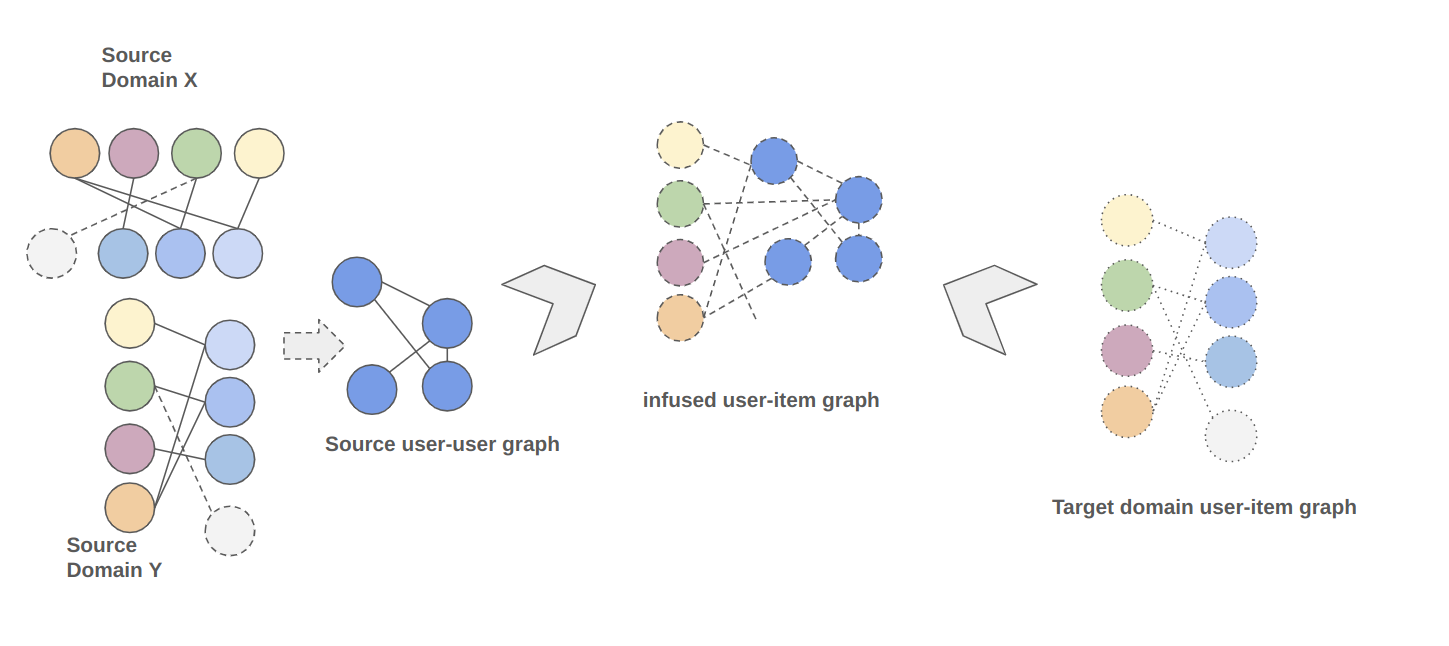
\includegraphics[width=1\textwidth]{figs/multi-graph-fusion.png}
    \caption{Illustration of the proposed method: The source domain data is first augment from user-item graph into a user-user graph. Then the augmented source user-user graph is then adapted into the target domain as a subgraph. finally the model is trained on the infused graph in a coherent way.}
    \label{fig:source-target-transfer}
\end{figure}

Leveraging information from other domains to enrich user and item representations in the target domain. However, some source domains frequently suffer from data sparsity issues themselves, introducing unwanted noise and reducing the effectiveness of the source data. Hence in our approach, we focuses on both the effectiveness and efficiency when transferring information from the source domain to the target domain. We first structure the bipartite graph for target domain, where the user and item nodes are connected by the interactions. Next, we leverage graph augmentation on source domain data, the augmented graph brings a number of benefits:

\begin{itemize}
    \item It can effectively improve graph density on shared nodes. (see more detailed comparison in section 4)
    \item Apply learnable edge regulation to adjust the edge weights based on the target domain data, which can effectively filter out the noises from the source domain data. e.g. reducing the impacts of highly connected nodes in the source domain, which may over weighted during the training process.
    \item user-user edges can be seamlessly integrated into the target domain graph, which can provide additional information for user representation learning.
\end{itemize}

We put adapt the augmented graph edges to the target domain by applying the edge regulation with a learnable weights.
The edge regulation is designed to adjust the edge weights based on the target domain data, which can effectively filter out the noises from the source domain data. e.g. reducing the impacts of highly connected nodes in the source domain, which may over weighted during the training process.
Finally, source and target domain data would be put through a GNN model to learn the user and item representations.
We use BPR as the optimization objective for training.
The user and item representations are learned jointly, thus, the information from the source domain is used to improve the target domain recommendation performance.
infuse target and source domains into a unified graph structure also improve the computational efficiency with less parameters to train, comparing to multi-graph approaches.

\subsection{Graph Construction for Target Domain}


\begin{figure}
    \centering
    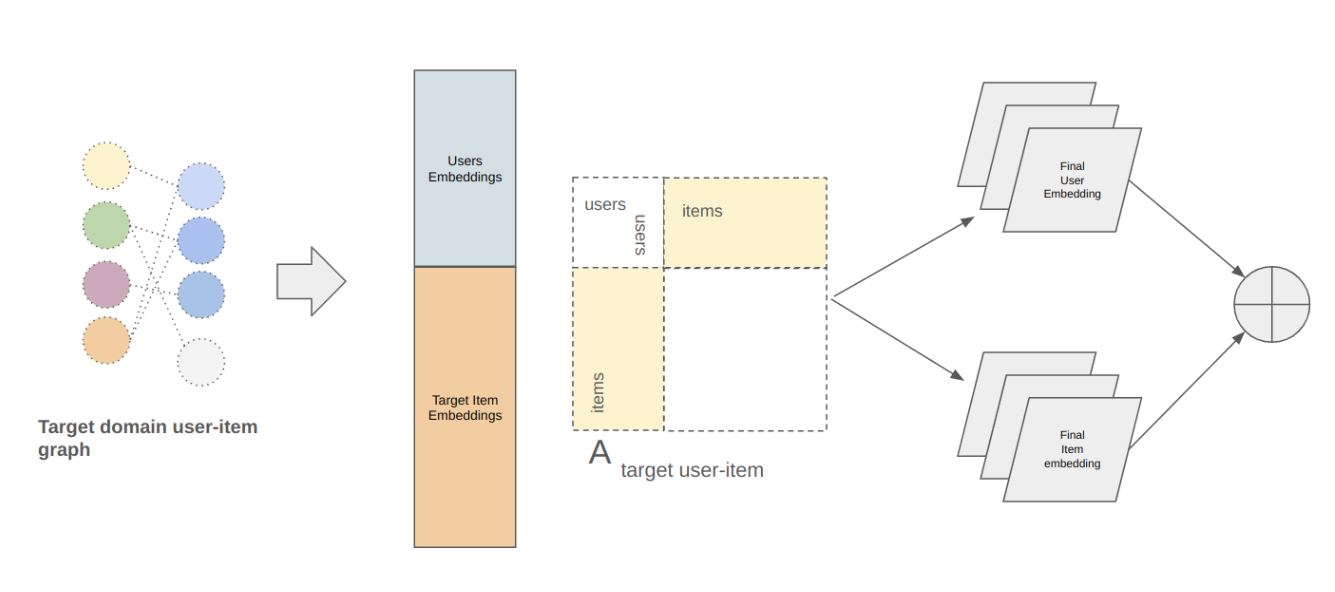
\includegraphics[width=1\textwidth]{figs/target-domain-graph.png}
    \caption{Illustration of LightGCN aggregator on target domain.}
    \label{fig:lightgcn}
\end{figure}


We define the domain user-item interactions as:
\begin{equation}
\centering
G = (V_{user/item}, E_{interaction})
\end{equation}

Where $V_{user/item}$ are the user and item nodes, and $E_{interaction}$ are the interactions between users and items in target Domain.

User and Item nodes presentation are learned using Graph Neural Network (GNN) model via nodes messaging and layer aggregation.

The basic GNN model aggregation can be abstract as:

\begin{equation}
\centering
e_u^{(k+1)} = AGG(e_u^(k),{e_i^(k), i \in N(u)})
\end{equation}

AGG can be different implementations of Aggregator such as GCN \cite{kipf2016semi, veličković2018graphattentionnetworks, hamilton2017inductive} are commonly used in GNN models.
The AGG function is the core of how message being propagated via nodes and its neighbors throughout the graph topology.
Those aggregators are designed to learn the node representation by using non-linear activation functions in feature transformation. Its effectiveness is proven in many classifier tasks.
However, when it comes to recommendation tasks, especially, when user interaction are only training dataset available.
The aggregator with nonlinearity functions commonly leads to over-smoothing issue, leads to poor performance and low variations in recommendation tasks \cite{Sharma2023ExperimentalHA}.

On the other hand, the aggregator, such as, LightGCN \cite{he2020lightgcn}, has proven results on improving the recommendation performance by adopting simple weighted sum aggregations, while reducing computation intensity at the same time.
During our experiments, we also found that LightGCN being more superior handling the over-smoothing issue, comparing to former mentioned aggregators.


In our approach, we construct the target domain graph as following.
we define a feature matrix for both user and item as E, while the adjacency matrix is defined as the user-item interaction matrix R=$R \in \mathbb{R}^{M \times N}$, where $M$ and $N$ are the user and item size.
hence the adjacency matrix can be presented as:

\begin{equation}
    E_{N+M} = \begin{pmatrix}
    E_{users} \\
    E_{items}
    \end{pmatrix},
    \quad
    A = \begin{pmatrix}
        0, & R_{N \times M} \\
        R^T_{M \times N}, & 0
        \end{pmatrix}
\end{equation}




hence, if we put the target domain through LightGCN aggregator:
\begin{equation}
E^{k+1} = (D^{-1/2} A D^{-1/2}) E^{k}
\end{equation}

We can get final user and item representation $e_{user}, e_{item}$ as:
\begin{equation}
    e_{user} = \sum_{l=0}^K \alpha_l e^{(l)}_{user};    \quad   e_{item} = \sum_{l=0}^K \alpha_l e^{(l)}_{item}
\end{equation}

where K is the number of layers in the GNN model, and $\alpha_l$ is the learnable weights for each layer.


\subsection{Source Domain Graph Augmentation}

\subsubsection{User-User Graph Augmentation}

\begin{figure}
    \centering
    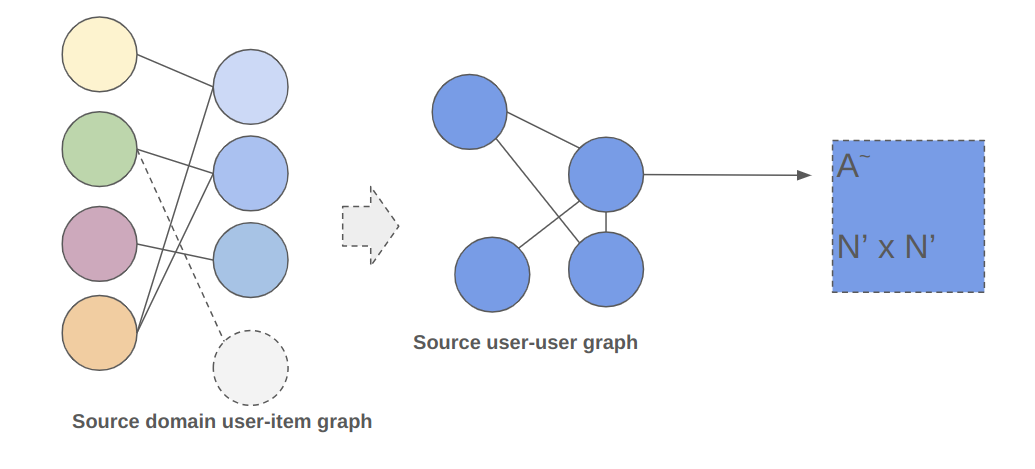
\includegraphics[width=1\textwidth]{figs/source-domain-graph.png}
    \caption{Illustration of the source domain user-user graph.}
    \label{fig:source-domain-graph}
\end{figure}

On the source domain side, we can derive the user-user or item-item graphs, based on common user/item interactions they share. (for simplicity, for the rest of the paper, we will use user-user graph as an example, the same logic can be applied to item-item graph as well.)

Say, the source domain has a user number of $N^{'}$ over lapping with the target domain $ N \cap N^{'}  >0 $. The source user-user graph presented as User Feature Embedding $E_{s}$, and the user-user interaction matrix $R_{s}$.:

\begin{equation}
    E_{s} = \begin{pmatrix}
    E_{N^{'}} \\
    \end{pmatrix},
    \quad
    A_{s} = \begin{pmatrix}
       R_{N^{'} \times N^{'}}
        \end{pmatrix}
\end{equation}

Apply degree normalization to the source user-user graph with weighted edges:

\begin{equation}
    A\tilde{~}_{s_ij} = \frac{ w_{s_ij}}{\sqrt{d_{s_i}} \sqrt{d_{s_j}}}
\end{equation}

The goal is remove the unuseable item nodes from the source. improving the density of the user-user graph, so the user similarity can be better learned and transferred to the target domain.


\subsubsection{Adapt Source Domain to Target Domain}

We adapt the source user-user adjacency matrix to the target domain user-item adjacency matrix.
Thus we get:

\begin{equation}
A_{infused} = \begin{pmatrix}
    0 + \begin{pmatrix}
        R_{N^{'} \times N^{'}}
        \end{pmatrix}, & R_{N \times M} \\
    R^T_{M \times N}, & 0

\end{pmatrix}
\end{equation}

Source User Feature Embedding $E_{s}$ will be shared with the target domain user feature embedding $E_{user}$, during training.

\begin{figure}
    \centering
    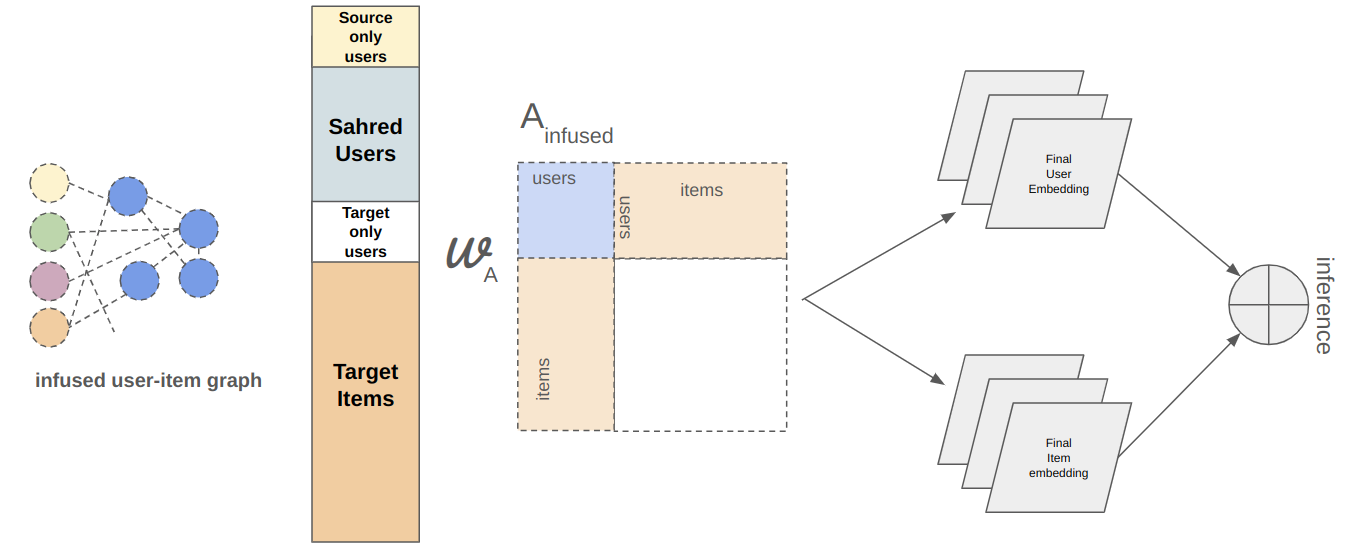
\includegraphics[width=1\textwidth]{figs/infused-domain-graph.png}
    \caption{Illustration of the source domain graph infusion to the target domain.}
    \label{fig:source-target-infusion}
\end{figure}

As we can see, during this process, fresh new users from the source, used to be out of target domain matrix, get introduced into the target domain from source. This enables the final model to make recommendation for those pure cold users, even no user-item interaction data is available in the target domain.
more details will be discussed in the experiment section.


\subsection{Model Training and Optimization}

\subsubsection{Source Domain Transfer Comparison}
Comparing to other source domain transfer methods, in general, we see the learning transfer is done via some form of dual or multi targets learning as model optimization objective.

A simplified loss function can be presented as:
\begin{equation}
    \begin{aligned}
        &\hat{y} = f_{target}(x_{target}) \\
        &\hat{y}^{'} = f_{source}(x_{source}) \\
        &L = L_{target} + L_{source} + \lambda L_{reg}
    \end{aligned}
\end{equation}

where $f_{target}$ and $f_{source}$ are the target and source domain models, $L_{target}$ and $L_{source}$ are the loss functions for target and source domain, and $L_{reg}$ is the regularization term.

CoNet \cite{Hu_2018} employs dual knowledge transfer across domains by introducing cross connections from one base network to another. Similarly, several other cross-domain recommender systems, such as PPNG \cite{zhao2019cross} and DTCDR \cite{DTCDR2019zhu}, adopt a similar approach with minor differences in their loss objectives, despite significant variations in their model architectures. In RecSys-DAN \cite{wang2019recsys}, transfer learning is achieved using a domain adversarial network.

A common aspect of these models above, are, all source embeddings are learned as part of the training process for knowledge transfer and domain alignment. Although these source domain embeddings are not used for the final recommendations, they still introduce additional parameters to train, increasing the model complexity.

\subsubsection{Simplified Taining Objective}

In our approach, we only use the source domain data to augment the target domain graph, hence no "waste" on the embedding learning for the model training. Thus, significantly reduces the model complexity and computational cost.

The trainable parameters in the model are the user and item embeddings, and the edge weights in the infused graph. the over lapped user between the source and target domain shares the same embeddings in the model.

We use Bayesian Probability Ranking as our optimization objective:

\begin{equation}
    L_{BPR} = -\sum\limits_{(u, i, j) \in E} \log \sigma(e_u \cdot e_i - e_u \cdot e_j)+  \lambda||E||^2
\end{equation}

Where $\sigma$ is the sigmoid function, $E$ is the set of user/item embeddings, $e$ is the embedding out put from the final layer. the $i$ and $j$ are the positive and negative samples for user $u$.
We use the L2 regularization, and the model is trained using Adam optimizer in mini batches.
